% !TEX TS-program = xelatex
% !TEX encoding = UTF-8 Unicode
% !TEX spellcheck = de_DE
% 
% © 2015–2017 Moritz Brinkmann, CC-by-sa
% http://latexkurs.github.io

\documentclass[
	vorläufig=true, 
	blattnr=5,
	ausgabe=2017-11-24,
	abgabe=2017-12-01,
	lösung=false,
	shortverb,
]{../tex/latexkurs-exercise}

\usepackage{mathtools, siunitx, booktabs}
\newcommand\zeit[2]{#1\textsuperscript{#2}}


\begin{document}


\begin{aufgabe}[6]{Abbildungen}
Üben Sie den Umgang mit Abbildungen und Grafiken in einem Dokument anhand der folgenden Unteraufgaben:
	\begin{enumerate}[label=\alph*)]
		\item Schreiben Sie zunächst den Code, um ein Bild in ein Dokument einzufügen und testen Sie,
ob das Bild im pdf zu sehen ist. Sie können ein beliebiges Bild verwenden, das in einer |figure|-Umgebung stehen sollte.
		\item Testen Sie den Einfluss von Parametern bei der Bildeinbindung, speziell Parameter zur
Skalierung und Rotation der Bilder. Geben Sie im fertigen Dokument mindestens zwei
Parameter an.
		\item Binden Sie nun ein weiteres Bild ein und verwenden Sie eines der „sub“-Pakete (\pkg{subcaption}, \pkg{subfloat}), damit beide Abbildungen eine einheitliche Numerierung bekommen (Abbildung 1a, Abbildung 1b o.\,ä.). Beide Bilder sollen sich dabei in einer Gleitumgebung befinden.
	
		Verwenden Sie zwei beliebige Bilder, jedes Bild soll dabei eine eigene Unterschrift bekommen; falls nötig, setzen Sie noch eine Gesamtbeschriftung für beide Bilder.
		\item Erweitern Sie Ihr Dokument abschließend um Text, den Sie mittels des |\blindtext|-Befehls aus dem \pkg{blindtext}-Paket eingeben. Denken Sie an das Laden von \pkg{babel} oder \pkg{polyglossia} und eine Sprachangabe!
		\item Schreiben Sie vor und hinter die Abbildungen Text und testen Sie die Endausgabe, wenn Sie Parameter an die figure -Umgebungen anhängen (|[h]|, |[b]| oder |[t]|). Welche Effekte beobachten Sie? Notieren Sie dies handschriftlich auf Ihrer Abgabe.
	\end{enumerate}
	\abgabe{Quellcode per Mail, Quellcode und fertiges Dokument ausgedruckt.}
\end{aufgabe}

\lösung{05_loesung_subcaption}
\clearpage

\begin{aufgabe}[6]<6>{Baum mit \TikZ }
	Das Makropaket \pkg{PGF} bietet mit dem Frontend \pkg{TikZ} eine hervorragende Möglichkeit, qualitativ hochwertige Grafiken mit \TeX\ zu erstellen. In dieser Aufgabe sollen Sie sich ein wenig mit \TikZ befassen. Aufgrund der Vielseitigkeit und des Umfangs von \TikZ beschränken wir uns darauf einen Baum mit \TikZ zu malen. Bäume eignen sich, um hierarchische Daten darzustellen und kommen zum Beispiel in der Informatik häufig zum Einsatz.

	\begin{enumerate}[label=\alph*)]
		\item Erstellen Sie eine |tikzpicture|-Umgebung, in der Sie einen Baum anlegen. Konsultieren sie dazu die \TikZ-Dokumentation\footnote{|texdoc tikz|, durchsuchen Sie das Dokument nach „trees“.} oder suchen Sie im Internet nach Beispielen für Bäume. Ihr Baum soll mindestens den Umfang des Baums in Abbildung \ref{fig:tree} haben.
	\end{enumerate}
		Die folgenden Aufgaben sind freiwillig und Sie müssen nur diejenigen bearbeiten, von denen Sie glauben, dass Sie Ihnen Spaß machen, oder Sie etwas lernen werden. Sie können für die Bearbeitung bis zu 6 Bonuspunkte erhalten.
	\begin{enumerate}[resume, label=\alph*)]
		\item Ergänzen Sie Ihren Baum um weitere Ebenen und Verzweigungen. Achten Sie dabei darauf, dass sich die Beschriftungen der einzelnen Knoten nicht überschneiden und passen Sie die Abstände entsprechend an. Falls nötig können sie auch die gesamte Darstellung des Baums ändern und ihn z.\,B. nach rechts statt nach unten wachsen lassen.
		
		Wenn Ihnen Bierstile nicht ergiebig genug sind, können Sie mit Ihrem Baum auch etwas (beliebiges) anderes darstellen. Sie sollten nur keinen Baum abgeben, der weniger Ebenen und Knoten enthält als der in Abbildung \ref{fig:tree}.
		
		\item \TikZ bietet – wie viele \LaTeX-Pakete – die Möglichkeit, die Darstellung von etwas völlig zu verändern, ohne den Inhalt dafür bearbeiten zu müssen.
		
		Geben Sie Ihrem Baum ein ansprechendes Aussehen! Setzen Sie zum Beispiel Farben ein, oder zeichnen Sie Formen um die einzelnen Knoten. Wenn Sie Lust haben, können Sie sich mal die |mindmap|-Library ansehen und Ihren Baum damit in ein organisches Gebilde verwandeln. Wenn Sie durch die \TikZ-Anleitung scrollen, werden Sie viele Anregungen finden.
		
		Die Art und Weise Ihrer Darstellung sollte dabei aber zum Inhalt passen und nicht von ihm ablenken.
	\end{enumerate}
	
	\abgabe{Quellcode per Mail, Quellcode und fertiges Dokument ausgedruckt.}
\end{aufgabe}

	\begin{figure}[]
		\centering
		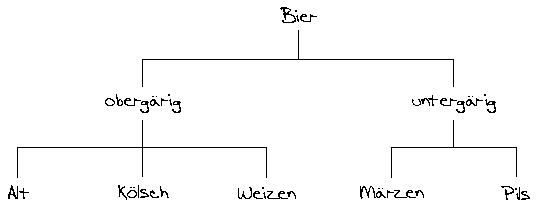
\includegraphics{05_tree}
		\caption{Stammbaum einiger Bierstile}
		\label{fig:tree}
	\end{figure}

\lösung{05_loesung_tree}



\end{document}